\section{Practical Algorithm: MeLU for Cold-Start Recommendation}

Recommendation is one of the most important services to Internet giants like TikTok, Taobao, etc. Where to put clients' advertisement to achieve the best efficiency and how to deliver end user their probably favoured products is of vital importance. Nowadays, with the thriving of artificial intelligence and ML algorithms, industries tend to utilize machine learning approach to support recommendation service. Cold start problems, however, is a critical problems that needs to be addressed for ML-based recommendation systems. When the number of user is still small, how to learn quickly and  provide recommendations accurately based on the statistics given. Or, when a new user come, how to quickly generate a home page of products or videos that the user may pay more attention to. Some classic algorithms like collaborative filtering might also be applied. Unlike the system based on collaborative filtering (the latter has similar ratings to the target user with other users), the proposed system only considers the products consumed by the target user.

In order to avoid user privacy issues during cold starts, many web-based systems (such as Netflix) recommend items based on minimal user information only. Netflix initially showed popular movies and TV shows to new users: we call these videos as candidate products. Then, the user selects his/her favorite video from the candidates. After that, the system will recommend some programs based on the video selected by the user. Recently, in order to improve performance, recommendations have been made using deep learning methods. However, for new users who only rated a few items, the cold start problem still exists.

To solve the cold-start problem of recommendation,one can use meta-learning approach like MAML , because this is a typical few-shot learning scenario. A practical work presented by paper MeLU\cite{lee2019melu}, designs and implements a recommendation system based on MAML. 


\begin{figure}[H] 
    \centering 
    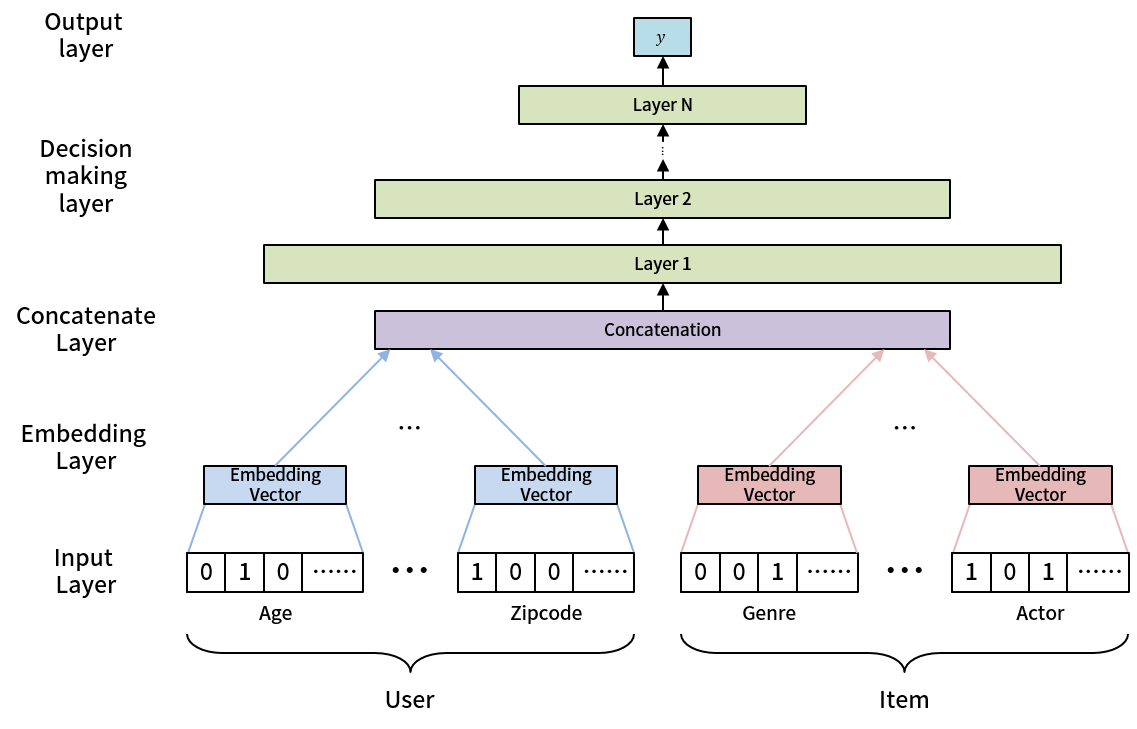
\includegraphics[width=0.7\textwidth]{image/MeLU-arch.png} 
    \caption{MeLU's User preference estimatior.}
    \label{fig:melu-estimator} 
\end{figure}

\subsection{MeLU's Method}
For user recommendation, MeLU first introduce a user preference estimator\ref{fig:melu-estimator} that consists of decision-making layers and output layer with user and item embeddings. MeLU model takes 

